%\newpage
%$ $
%\newpage

\renewcommand{\thesubsection}{\textcolor{red}{\Roman{section}.\arabic{subsection}}}
\renewcommand{\thesubsubsection}{\textcolor{red}{\Roman{section}.\arabic{subsection}.\alph{subsubsection}}}

\setcounter{section}{0}
\setcounter{document}{0}
\sndEnTeteTPDeux

\begin{center}
\begin{mdframed}[style=titr, leftmargin=60pt, rightmargin=60pt, innertopmargin=7pt, innerbottommargin=7pt, innerrightmargin=8pt, innerleftmargin=8pt]

\begin{center}
\large{\textbf{TP 2 : Mais qui a pollué la Seine ?}}
\end{center}

\end{mdframed}
\end{center}



\begin{tcolorbox}[colback=blue!5!white,colframe=blue!75!black,title=Objectifs de la séance :]
\begin{itemize}
    \item Mesurer une température de changement d'état,
    \item Réaliser une chromatographie sur couche mince,
\end{itemize}
\end{tcolorbox}

\begin{tcolorbox}[colback=orange!5!white,colframe=orange!75!black,title= Scénario:]
\og Le 5 août dernier, une compétition-test pré-JO de natation en eaux libres dans la Seine avait dû être annulée en raison de la pollution du fleuve.\fg 
\begin{flushright}
    \textit{Source : RadioFrance, le 16 août 2023}
\end{flushright}
\begin{large}
    \ding{43}
\end{large} Une grande usine est suspectée d’avoir déversé des milliers de litres de produits chimiques dans la Seine. Une équipe de scientifique a permis par évaporation d'isoler un solide blanc présent dans l'eau et un colorant. Vous avez pour mission de déterminer qui a déversé ces produits chimiques.
\end{tcolorbox}
\begin{center}
    \textbf{\textcolor{red}{Vous présenterez en fin de TP votre rapport d'enquêteur au professeur.}}
\end{center}

\section{Analyse d'une espèce solide}

\begin{doc}{Utilisation du banc Kofler}
Le banc Kofler est une plaque chauffante présentant un gradient de température, c’est à dire une augmentation progressive de la température de droite (température ambiante) à gauche (environ 250$\degreCelsius$-300$\degreCelsius$ selon les bancs). \textbf{Le banc Kofler permet de déterminer la température de fusion d’une espèce chimique}.
\begin{center}
    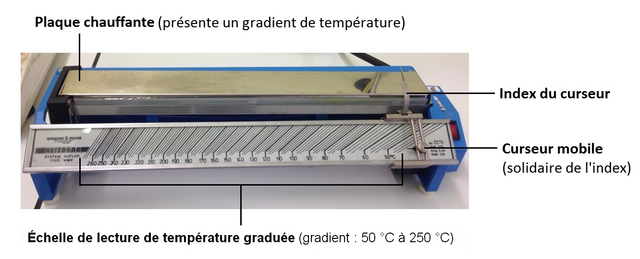
\includegraphics[scale=0.65]{Images/Chapitre_1/Banc_Kofler.png} 
\end{center}

Avant toute utilisation, le banc doit être étalonné (c’est-à-dire calibré). Voici les étapes d'utilisation du banc Kofler :
\begin{enumerate}
    \item \textbf{Etalonnage} \textit{(réalisé par le professeur)} : une très petite quantité de l’espèce étalon est déposée sur la partie froide du banc. On déplace ensuite cette quantité vers la partie chaude jusqu’à observer sa fusion. Le curseur de température est alors ajusté pour faire correspondre son index avec la température de l’étalon. Le banc doit ensuite être essuyé, pour enlever tous les résidus.
    \item \textbf{Mesure :} Comme lors de l’étalonnage, une petite quantité de l’espèce est déposée sur la partie froide du banc. On déplace ensuite cette quantité vers la partie chaude jusqu’à observer sa fusion. On lit à l’aide du curseur la température de fusion.
\end{enumerate}
Voici le lien d'une vidéo sur l'utilisation du banc : \url{https://ladigitale.dev/digiview/#/v/630614d1b4375}\\
\importantbox{Ne pas utiliser de gants lors de l'utilisation du banc Kofler !}
\end{doc}

\begin{doc}{Schéma des entreprises en bordure de la Seine}
\begin{center}
    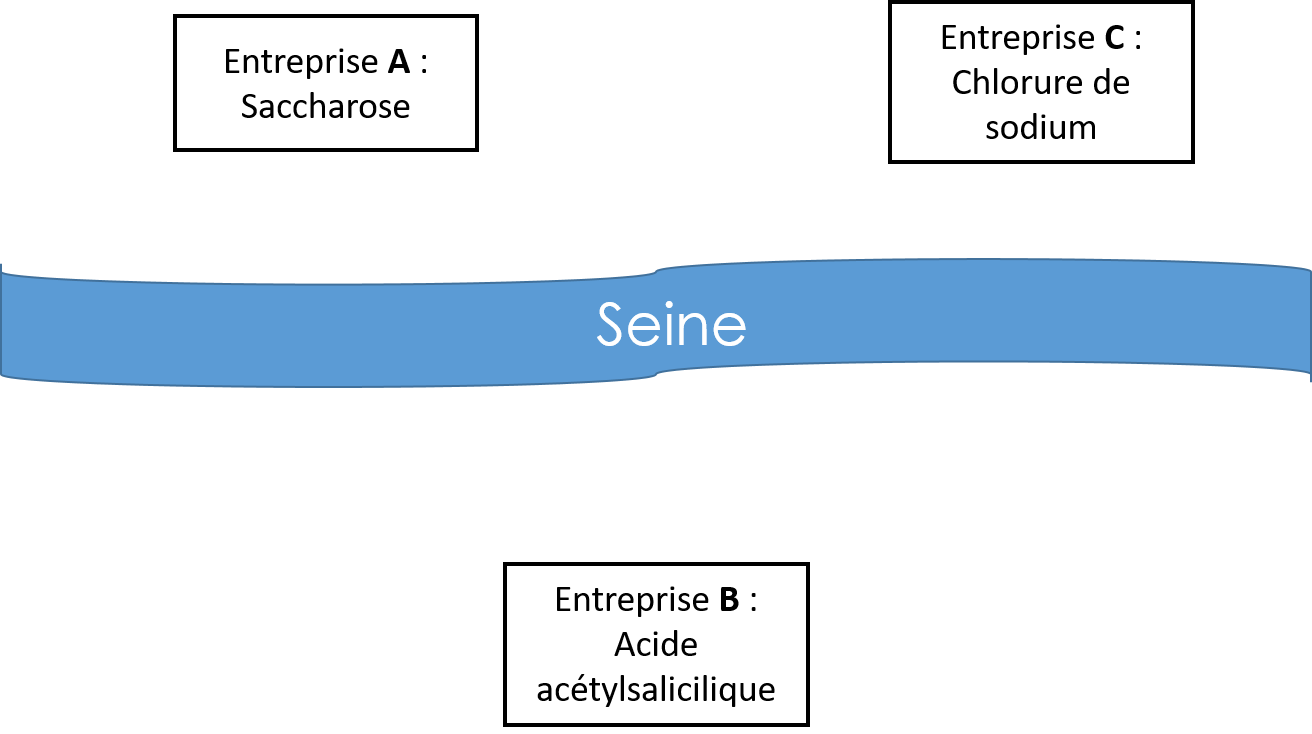
\includegraphics[scale=0.5]{Images/TP2/Entreprise.png}
\end{center}
\end{doc}
\newpage
\begin{doc}{Fiche technique des trois produits chimiques fabriqués par les entreprises}
\newline
    \begin{tabular}{|C{0.4}|C{0.1}|C{0.2}|C{0.2}|}
    \hline
     & Chlorure de sodium & Saccharose & Acide acétylsalycilique \\
    \hline
    Température de fusion $T_{f}$ \newline (en $\degreCelsius$) & 801 & 185,5 & 135 \\
    \hline
    Température d'ébullition $T_{eb}$ \newline (en $\degreCelsius$) & 1465 & Décomposition & Se décompose à 140 $\degreCelsius$ \\
    \hline
    Masse volumique (en g.cm$^{-3}$) & 2,16 & 1,59 & 1,4 \\
    \hline
    \end{tabular}
\end{doc}

\textbf{Vous souhaitez déterminer l’entreprise d’où provient la poudre retrouvée sur la victime pour en déduire ainsi le lieu du crime.}\\
A l’aide des documents :
\begin{enumerate}
    \item Trouver et rédiger le protocole à mettre en place
    \item Réaliser l’expérience
    \item Déterminer le lieu du crime en justifiant,
    \item \textit{(Bonus)} Proposer une autre technique qui aurait pu permettre de déterminer le lieu du crime
\end{enumerate}

\section{Analyse d'un colorant}
Maintenant que vous avez découvert le lieu du crime, les enquêteurs penchent sur deux suspects : le Professeur Violet qui utilise les colorants E102 et E131 et le Docteur Orchidée qui utilise le colorant E133.\\

\begin{doc}{Mettre en place une Chromatographie sur Couche Mince (CCM)}
Protocole expérimental :
    \begin{itemize}
        \item Introduire l’éluant (eau + éthanol) dans la cuve à chromatographie (sur environ 0,5 cm de hauteur). Fermer la cuve avec son couvercle pour la saturer en vapeurs d’éluant.
        \item Tracer, au crayon, sur le papier filtre la ligne de dépôt à 1,5 cm du bord inférieur. Placer, en les espaçant d’au moins 1 cm, une marque par dépôt à effectuer (ici 4 dépôts, \textbf{notez les sur le papier filtre !}),
        \item Déposer les échantillons à analyser à l’aide d’un tube capillaire. Un dépôt pour le feutre, un dépôt pour la tâche, un dépôt pour l’encre.
        \item Introduire la plaque dans la cuve (attention, la ligne de dépôt et les échantillons ne doivent pas être immergés dans l’éluant !) 
        \item Retirer la plaque à chromatographie de la cuve lorsque l’éluant a migré jusqu’à atteindre 1 cm du bord supérieur. Tracer au crayon le front de solvant.
    \end{itemize}
Une animation pour réaliser une CCM est disponible à cette adresse \url{https://ladigitale.dev/digiplay/#/v/63061cea42993} 
\end{doc}
%\qrcode{https://ladigitale.dev/digiplay/#/v/63061cea42993}
\begin{doc}{Analyse comparative d'un ou plusieurs chromatogrammes}
\begin{wrapfigure}{r}{0.4\textwidth}
\vspace{-1cm}
    \centering
      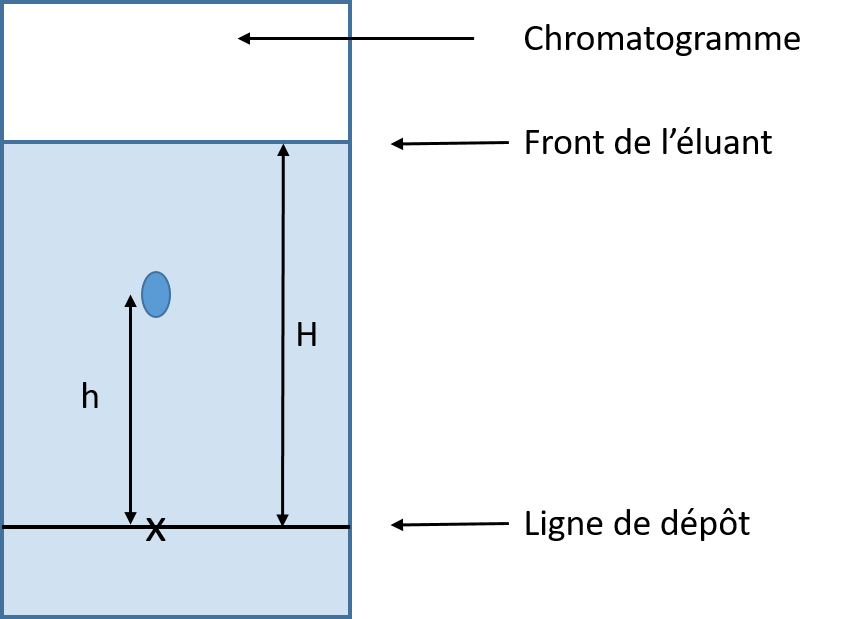
\includegraphics[width=0.4\textwidth]{Images/TP2/Chromatogramme.png}
  \end{wrapfigure}
    Le rapport frontal (noté $R_f$) se calcule à l'aide de la formule suivante :
\begin{equation*}
    R_f = \frac{h}{H}
\end{equation*}
avec $h$ la distance parcourue par l'espèce chimique, $H$ la distance parcourue par le front de l'éluant.\\
\textbf{Si deux espèces chimiques ont le même rapport frontal, alors elles sont identiques.}

\end{doc}



\begin{mdframed}[style=autreexo]
\textbf{\bsc{Liste du matériel}}
\begin{itemize}
    \item tube capillaire,
    \item flacon de colorant E133 ;
    \item flacon de colorant E102 ;
    \item flacon de colorant E131 ;
    \item papier filtre ;
    \item cuve chromatographique ;
\end{itemize}
\end{mdframed}
A l’aide des documents :
\begin{enumerate}
    \item À l’aide d’un schéma, présenter les résultats de la CCM,
    \item Interpréter les résultats de la CCM,
    \item Déterminer le coupable.
\end{enumerate}